\documentclass{beamer}
\usetheme{Copenhagen}
\usecolortheme{beaver}
\usepackage[utf8]{inputenc}
\usepackage{graphicx}
\usepackage{tcolorbox}
\usepackage[framemethod=TikZ]{mdframed}

\newcommand\Wider[2][3em]{%
	\makebox[\linewidth][c]{%
		\begin{minipage}{\dimexpr\textwidth+#1\relax}
			\raggedright#2
		\end{minipage}%
	}%
}

\newcommand\Wide[2][1.5em]{%
	\makebox[\linewidth][c]{%
		\begin{minipage}{\dimexpr\textwidth+#1\relax}
			\raggedright#2
		\end{minipage}%
	}%
}

\mdfdefinestyle{MyFrame}{%
	linecolor=blue,
	outerlinewidth=1pt,
	roundcorner=20pt,
	innertopmargin=\baselineskip,
	innerbottommargin=\baselineskip,
	innerrightmargin=10pt,
	innerleftmargin=10pt,
	backgroundcolor=gray!50!white}


\makeatletter
\setbeamertemplate{footline}
{
	\leavevmode%
	\hbox{%
		\begin{beamercolorbox}[wd=0.75\paperwidth,ht=2.25ex,dp=1ex,left]{title in head/foot}%
			\usebeamerfont{title in head/foot}\insertshorttitle{}
		\end{beamercolorbox}%
		\begin{beamercolorbox}[wd=0.25\paperwidth,ht=2.25ex,dp=1ex,right]{date in head/foot}%
			\insertframenumber{} / \inserttotalframenumber\hspace*{2ex} 
		\end{beamercolorbox}}%
		\vskip0pt%
}
\makeatother
 
 
%Information to be included in the title page:
\title[Clustering Documents]{Topic Modeling:}
\subtitle{from a Network Perspective}
\author{Cindy Cook}
\institute{Network Analysis: Presentation}
\date{26 April 2016}
 

\begin{document}
 
\frame{\titlepage}
 
\begin{frame}
	\frametitle{Outline}
 	\begin{enumerate}
 		\item Overview of Topic Modeling 
 		\vspace{2mm}
 		\item Replication of Paper
		 \vspace{2mm}
		 \item Data Sets
		 \vspace{2mm}
		 \item Extension 
 	\end{enumerate}
\end{frame}
 
\begin{frame}
	\frametitle{Topic Modeling:  The General Idea}
\Wide{
	\scriptsize
	\begin{itemize}
		\item[] \hspace{-3.5mm}1. Obtain documents, $D$ and have an idea as to the number of topics $K$ within $D$.  
	\end{itemize}
	\vspace{-3mm}
	\begin{columns}
		\column{0.5\textwidth}
		\scriptsize
		\begin{itemize}
		\item[] 2. Stem and remove stop words. 
		\item[] 3. Create the term-frequency matrix.
		\item[] 4. Apply model: LDA, pLSA, etc... 
		\item[] 5. Obtain:
		\begin{itemize}
			\scriptsize
			\item[] a) For each $d,$ a topic distribution.
			\item[] b) For each topic $k,$ a word distribution. 
		\end{itemize}
		\end{itemize}
		\column{0.5\textwidth}
		\begin{mdframed}[style=MyFrame]
			
		Example:
		\vspace{-2mm}
			\begin{align*}
			d1:& \text{I \textcolor{red}{like} to \textcolor{red}{eat} \textcolor{red}{fish} for \textcolor{red}{dinner}.} \\
			d2:& \text{I only \textcolor{red}{eat} \textcolor{red}{ice} \textcolor{red}{cream} after \textcolor{red}{dinner}.} \\
			d3:& \text{I \textcolor{red}{own} a \textcolor{red}{pet} \textcolor{red}{fish} \textcolor{red}{name}d \textcolor{red}{Nemo}.}
			\end{align*}
		\end{mdframed}	
\end{columns}
\vspace{-2mm}
	\begin{center}
		\tiny
		\textcolor{blue}{Term-Frequency Matrix}\hspace{15mm}\textcolor{blue}{Topic/Word Distributions} \\
		\begin{tabular}{ |c||c|c|c|||c|c||c|c|  }
			\hline
			&$d1$&$d2$&$d3$& $k1$& $k2$&$k1$&$k2$ \\
			\hline   
			\textcolor{red}{cream}&0&1&0& 0.0833&0&0.0825 &0.0714 \\
			\textcolor{red}{dinner}&1&1&0& 0.1666&0&0.1480 &0.1597\\
			\textcolor{red}{eat}&1&1&0& 0.1666&0&0.2710 &0.0369\\
			\textcolor{red}{fish}&1&0&1&0.0833&1&0.1509& 0.1568 \\
			\textcolor{red}{ice}&0&1&0&0.0833&0&0.0935 &0.0604 \\
			\textcolor{red}{like}&1&0&0&0.0833&0&0.0387 &0.1150 \\
			\textcolor{red}{name}&0&0&1&0.0833&0&0.0255 &0.1283 \\
			\textcolor{red}{nemo}&0&0&1&0.0833&0& 0.0809& 0.0729 \\
			\textcolor{red}{own}&0&0&1& 0.0833&0& 0.0253& 0.1285 \\
			\textcolor{red}{pet}&0&0&1&0.0833&0&0.0837& 0.0701 \\
			\hline
			$k1$& 0.5010&  0.5051& 0.4939&&&&\\
			$k2$&0.4990& 0.4949& 0.5061&&&&\\
			$k1$&0&0&0.8&&&&\\
			$k2$&1&1&0.2&&&&\\
			\hline
		\end{tabular}
	\end{center}
}
\end{frame}


\begin{frame}
	\frametitle{A Network Prespective:  TopicMapping}
\Wide{
	*Before step 4:\\
	\vspace{10mm}
		\hspace{2mm} \footnotesize{Bipartite Graph \hspace{26mm} Projected \hspace{30mm} Estimates}
	\vspace{-5mm}
		\begin{columns}
			\column{0.2\textwidth}	
			\tiny
			\textcolor{blue}{Term-Frequency Matrix} \\
			\begin{tabular}{ |c||c|c|c|  }
				\hline
				& d1& d2& d3 \\
				\hline   
				\textcolor{red}{cream}& 0& 1& 0 \\
				\textcolor{red}{dinner}& 1& 1& 0 \\
				\textcolor{red}{eat}& 1& 1& 0 \\
				\textcolor{red}{fish}& 1& 0& 1 \\
				\textcolor{red}{ice}& 0& 1& 0 \\
				\textcolor{red}{like}& 1& 0& 0 \\
				\textcolor{red}{name}& 0& 0& 1 \\
				\textcolor{red}{nemo}& 0& 0& 1 \\
				\textcolor{red}{own}& 0& 0& 1\\
				\textcolor{red}{pet}& 0& 0& 1 \\
				\hline
			\end{tabular} 
			\column{0.4\textwidth}	
			\begin{figure}[ht!]
				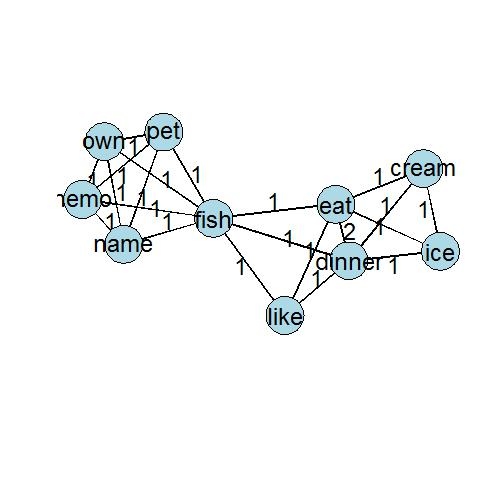
\includegraphics[width=40mm,height=40mm]{word_sp.jpeg}
			\end{figure}
			 \column{0.2\textwidth}
 			\tiny
 			\textcolor{blue}{Topic/Word Dists.} \\
 			\begin{tabular}{ |c||c|c|  }
 				\hline
 				& k1& k2 \\
 				\hline   
 				\textcolor{red}{cream}& 0.1667& 0 \\
 				\textcolor{red}{dinner}& 0.1667& 0 \\
 				\textcolor{red}{eat}& 0.1667& 0 \\
 				\textcolor{red}{fish}& 0.1667& 1 \\
 				\textcolor{red}{ice}& 0.1667& 0 \\
 				\textcolor{red}{like}& 0.1667& 0 \\
 				\textcolor{red}{name}& 0& 0.25 \\
 				\textcolor{red}{nemo}& 0& 0.25 \\
 				\textcolor{red}{own}& 0& 0.25\\
 				\textcolor{red}{pet}& 0& 0.25 \\
 				\hline
 			\end{tabular} 
		\end{columns}
		%\vspace{-3mm}
		\normalsize{*Replication Study:}
%		\begin{columns}
%		\column{0.4\textwidth}
%		\begin{itemize}
%			\item Theoretical Results
%			\item Simulations
%			\item Real World Applications
%		\end{itemize}
%			\column{0.6\textwidth}
%			\vspace{-10mm}
%			\begin{center}
%			\begin{figure}[]
%				\hspace{-4mm}
%				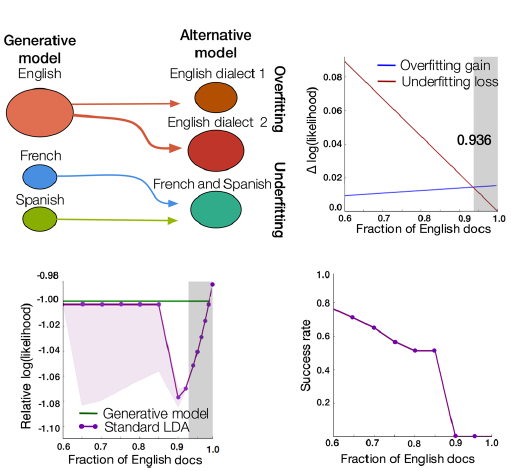
\includegraphics[width=30mm,height=30mm]{language_test2.png}
%				\hspace{5mm}
%				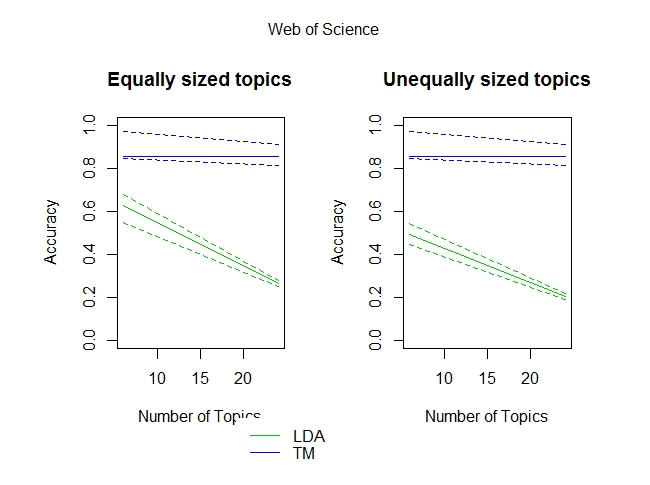
\includegraphics[width=30mm,height=30mm]{plot_WoS.jpeg}
%			\end{figure}
%			\end{center}
%		\end{columns}
}
\end{frame}


\begin{frame}
	\frametitle{Data}
\Wider{
	\footnotesize{	
	\begin{enumerate}
		\item[\textcolor{black}{1.}] Web of \textcolor{orange}{Science}: Each document includes the title and abstract of an article from different fields including economics, astronomy, psychology, biology, and math.
		\item[\textcolor{black}{2.}] \textcolor{cyan}{Indeed}.com: Each document includes past work experience for an individual in teaching, graphic, architecture, accounting, and nursing.
	\end{enumerate}	
	}
	%\begin{columns}
	%	\column{0.5\textwidth}
	%	\vspace{-3mm}
	%	\begin{figure}[ht!]
	%		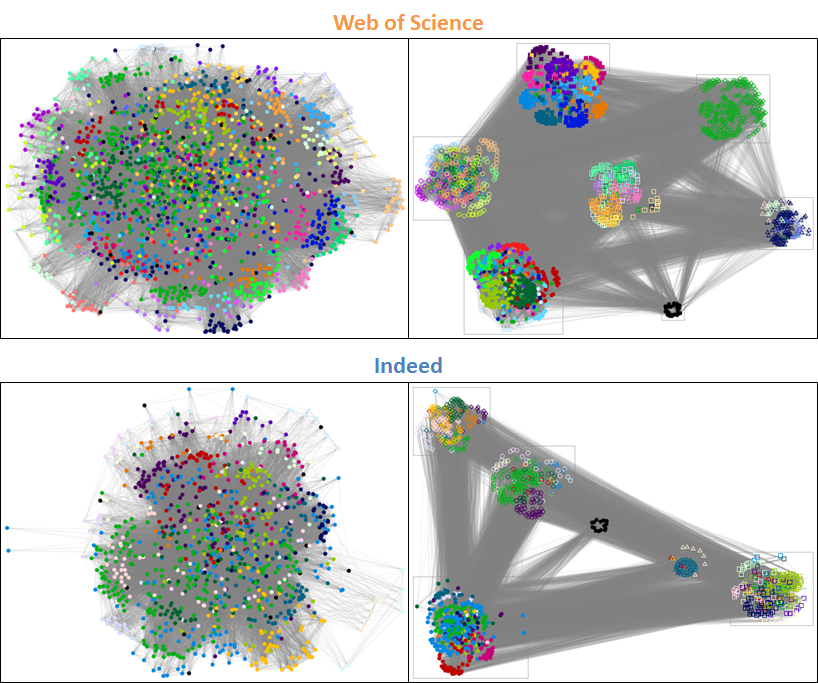
\includegraphics[width=60mm,height=50mm]{networks.png}
	%	\end{figure}
	%	\column{0.4\textwidth}
		\vspace{-3mm}
		\begin{figure}[ht!]
			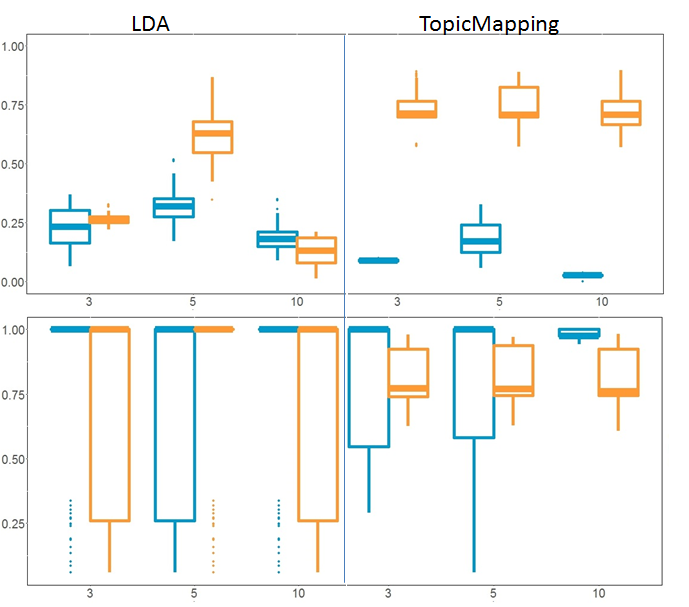
\includegraphics[width=80mm,height=50mm]{results.png}
		\end{figure}
	%\end{columns}
	
}
\end{frame}

\begin{frame}
	\frametitle{Network Comparison: Descriptive}
	\Wider{
	Modularity: 
	%	\begin{columns}
	%	\column{0.5\textwidth}	
	\begin{center}
		\footnotesize
		\begin{tabular}{ |c|c|c|  }
			\hline
			Clustering Type&\textcolor{orange}{Science}&\textcolor{cyan}{Indeed} \\ 
			\hline 
			InfoMap& 0.3884&0.3881 \\
			Fast-Greedy& 0.3398& 0.3358\\
			Eigenvalue& 0.3624&0.3616 \\
			Louvain&0.3936&0.3904 \\
			Walktrap&0.3257&0.3431 \\
			\hline
		\end{tabular}
	\end{center}
	\vspace{2mm}
		Density, Transitivity, Betweenness Centrality, Degree Assortativity, \\
		Degree Distributions:
		\vspace{-2mm}
	\begin{figure}[H]
		\centering
		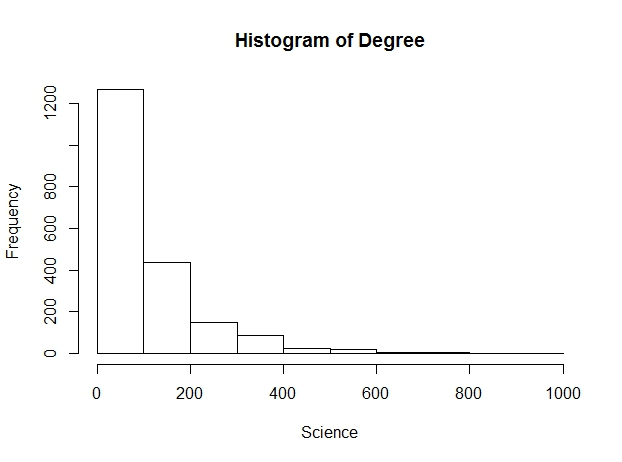
\includegraphics[scale=0.2]{degree_hist_sci.jpeg}
		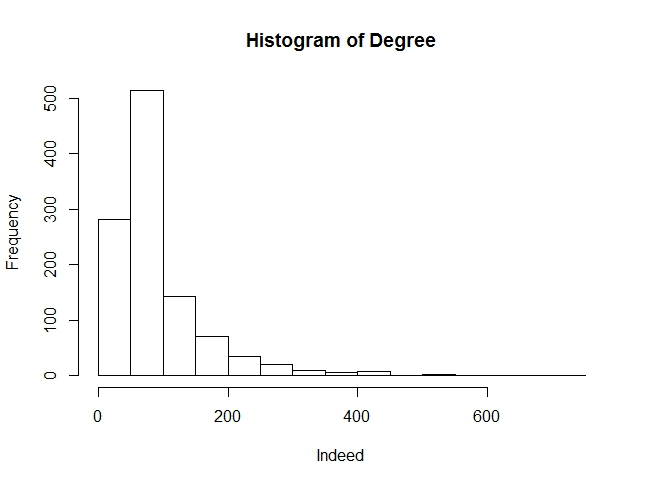
\includegraphics[scale=0.2]{degree_hist_ind.jpeg}
	\end{figure}

%	\column{0.5\textwidth}	
%		\begin{figure}[H]
%			\centering
%			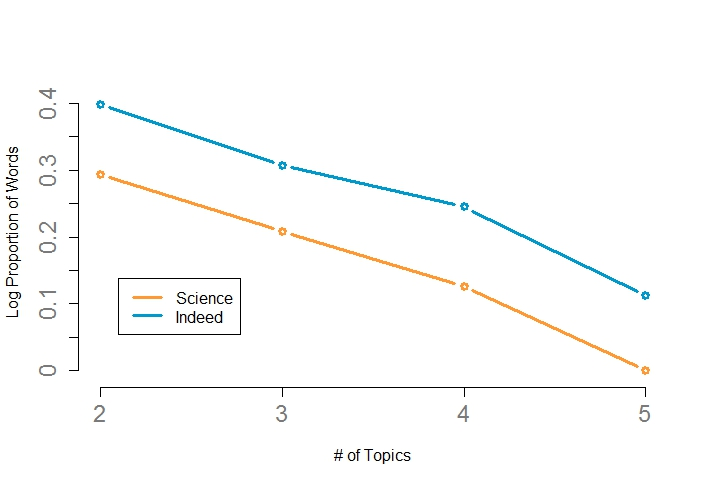
\includegraphics[scale=0.2]{props.jpeg}
%		\end{figure}
	%\end{columns}
	}
\end{frame}

\begin{frame}
	\frametitle{Network Comparison: Extension}
	\Wider{
	*\small{ERGM}
	\begin{center}
		\tiny	
		\begin{tabular}{ |c|c|c|c|c||c|c|c|c|c|c|  }
			\hline
			&\textcolor{orange}{Science}&&&&\textcolor{cyan}{Indeed}&&& \\
			\hline
			&Estimate&Std. Error&MCMC$\%$&p-value&Estimate&Std. Error&MCMC$\%$&p-value \\ 
			\hline 
			edges&-3.3591&0.0040&0&$<0.0001$&-2.9925&0.0063&0&$<0.0001$\\
			isolate&-Inf&0&0&$<0.0001$&-Inf&0&0&$<0.0001$\\
			homophily&3.3696&0.0077&1&$<0.0001$&3.3616&0.0122&0&$<0.0001$\\
			\hline
		\end{tabular}
	\end{center}
	*\small{QAP}
		\begin{center}
			\tiny	
			\begin{tabular}{ |c|c|c|c|c||c|c|c|c|  }
				\hline
				&\textcolor{orange}{Science}&&&&\textcolor{cyan}{Indeed}&&& \\
				\hline
				&Estimate&Pr$(\le b)$ &Pr$(\ge b)$ &Pr$(\ge |b|)$&Estimate&Pr$(\le b)$ &Pr$(\ge b)$ &Pr$(\ge |b|)$ \\ 
				\hline 
				intercept&0.0463& 1&   0&  0&0.0621& 1&       0&       0      \\
				Homophily&0.9537 &1  &0   &0&0.9379 &1       &0       &0\\
				\hline
				Adj. $R^{2}$&0.2406&&&&0.245&&& \\
				\hline
			\end{tabular}
		\end{center}
	*\small{CUG} \\
	\hspace{5mm} -\footnotesize{Conditional on each network's dyad distribution.} \\
	\hspace{10mm} \footnotesize{Modularity} \\
	\hspace{10mm} \footnotesize{Transitivity} 
}
\end{frame}


\end{document}